\documentclass[UTF8]{article}
\usepackage{ctex}
\usepackage{amsmath}
\usepackage{graphicx}
\begin{document}
\section{第四讲\;\;}
\subsection{功\;\;功能定理}
\subsubsection{功}

    (1)物体作直线运动,恒力做功
    \[A = Fcos\theta \cdot \lvert \Delta \vec{r} \vert\;\;\;\;\;A = \vec{F}\cdot\vec{\Delta r}\]

    (2)物体作曲线运动,变力做功
    \[\mbox{元功:}dA = Fcos\theta\cdot\lvert d\vec{r}\vert = \vec{F}\cdot d\vec{r}\]

    \[\mbox{总功:}A = \int_A^BdA = \int_A^B\vec{F}\cdot d\vec{r} = \int_A^BFcos\theta \lvert d\vec{r}\vert\]

    (3)质点同时受几个力作用时

    力的叠加原理:$\vec{F} = \vec{F_1} + \vec{F_2} + \dots + \vec{F_N}$

    \;\;\;\;\;\;\;\;\;\;\;\;\;\;\;\;\;\;\;\;$A = A_{1AB} + A_{2AB} + \dots + A_{NAB}$

    说明:

    \;\;(1)合力的功等于各分力沿同一路径所做功的代数和

    \;\;(2)计算力对物体做功时,必须说明是哪个力对物体沿哪条路径所做的功

\subsubsection{动能定理}

    1、定义:质点动能\[E_k = \frac{1}{2}mv^2\mbox{ 或者 }E_k = \frac{p^2}{2m}\]

    2、质点的动能定理\[A_{\mbox{合}AB} = E_{kB} - E_{kA} = \Delta E_k = \frac{1}{2}mv_B^2 - \frac{1}{2}mv_A^2\]

    \;\;合外力对质点所做的功(其它物体对它所做的总功)等于质点动能的增量

    3、质点系动能定理

    对n个质点组成的质点系:对每个质点分别使用动能定理
    \[\sum_{i=1}^n A_{i\mbox{外}} + \sum_{i=1}^n A_{i\mbox{内} = \sum_{i=1}^n E_{kiB} - \sum_{i=1}^n E_{kiA}}\]

    所有外力对质点系做的功和内力对质点系做的功之和等于质点系总动能的增量

    注意:内力能改变系统的总动能,但不能改变系统的总动量

\subsection{保守力与非保守力}

    两质点间的“一对力”做功之和等于其中一个质点受的力沿着该质点相对于另一质点所移动的路径所做的功

    沿任意回路做功为零的力,或做功与具体路径无关的力都称为保守力

    大多数定向力和有心力都是保守力

\subsection{势能\;\;势能曲线}

    1、势能

    势能:系统在任一位形时的势能等于它从此位形沿任意路径改变至势能零点时保守力所做的功

    \[\mbox{势能}\left\{
        \begin{aligned}
        \mbox{势能与参考系无关(相对位移)     } \\
        \mbox{相对量:相对于势能零点的         } \\
        \mbox{系统量:是属于相互作用的质点共有的}
        \end{aligned}
        \right.\]
    
    \[\mbox{几种势能}\left\{
        \begin{aligned}
        \mbox{引力势能:(无穷远处为零势能点)} E_p(r) = -G\frac{m_1m_2}{r}\\
        \mbox{重力势能:(高度为零为零势能点)} E_p(h) = mgh\\
        \mbox{弹性势能:(自然伸长为零势能点)} E_p(x) = \frac{1}{2}kx^2
        \end{aligned}
        \right.\]
    
    2、势能曲线

    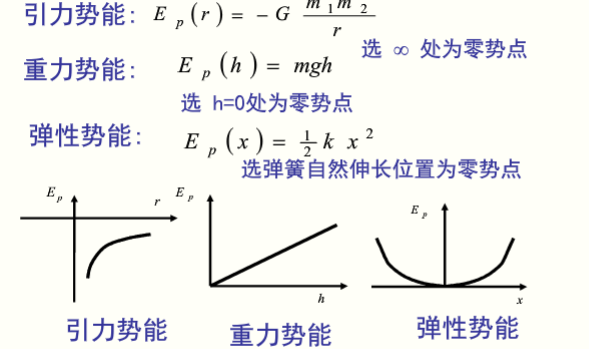
\includegraphics[width=13cm, height=8cm]{D:/UniversityNote/PhyNote/7.png}
    
    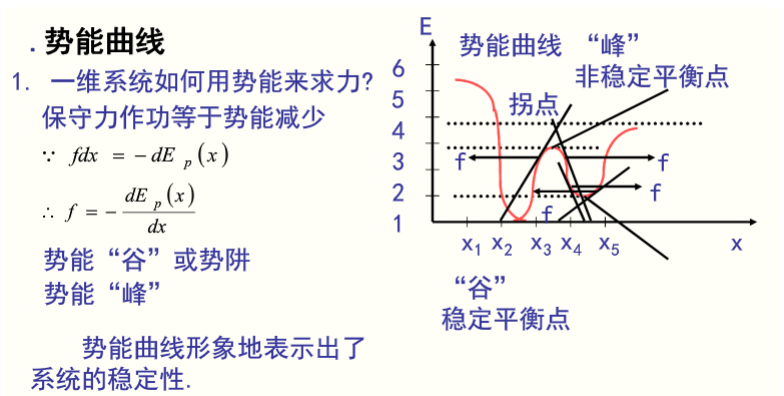
\includegraphics[width=13cm, height=8cm]{D:/UniversityNote/PhyNote/8.png}

    3、由势能求保守力

    梯度算符:$\bigtriangledown = \frac{\partial}{\partial x}\vec{i} + \frac{\partial}{\partial x}\vec{j} + \frac{\partial}{\partial x}\vec{k}$
    \[F_l = -\frac{dE_p}{dl}\;\;\;\;\;\vec{F} = -\bigtriangledown E_p\]

    保守力等于势能的负梯度

\subsection{功能原理以及机械能守恒定律}

    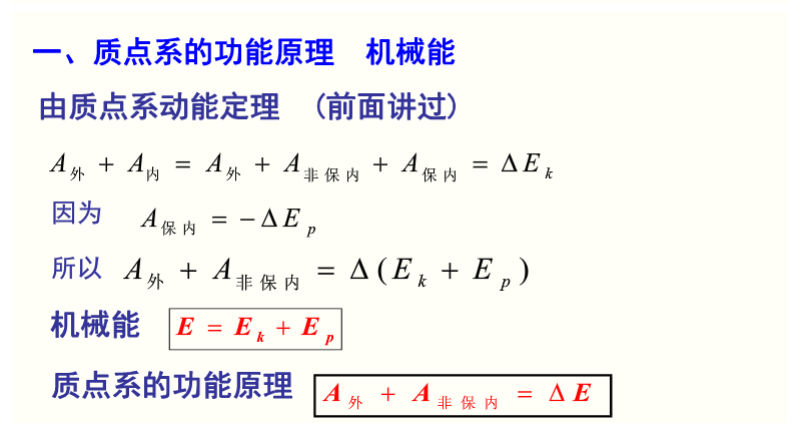
\includegraphics[width=13cm, height=8cm]{D:/UniversityNote/PhyNote/9.png}

    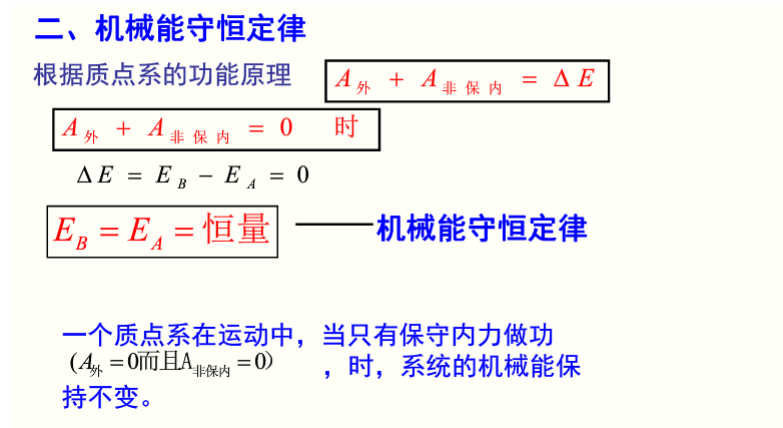
\includegraphics[width=13cm, height=8cm]{D:/UniversityNote/PhyNote/10.png}

\end{document}